\documentclass[a4paper]{article}
\usepackage[utf8]{inputenc}
\usepackage{fullpage}
\usepackage{csquotes}
\usepackage[ngerman]{babel}
\usepackage{biblatex}
\usepackage{float}
\usepackage{graphicx}
\usepackage{subfigure}
\usepackage[format=plain,labelfont=bf,up]{caption}
\usepackage{hyperref}
\usepackage{booktabs}
\usepackage{listings}
\usepackage{color}
\definecolor{lightgray}{rgb}{.9,.9,.9}
\definecolor{darkgray}{rgb}{.4,.4,.4}
\definecolor{purple}{rgb}{0.65, 0.12, 0.82}
\usepackage{array}

\lstdefinelanguage{JavaScript}{
  keywords={typeof, new, true, false, catch, function, return, null, catch, switch, var, if, in, while, do, else, case, break},
  keywordstyle=\color{blue}\bfseries,
  ndkeywords={class, export, boolean, throw, implements, import, this},
  ndkeywordstyle=\color{darkgray}\bfseries,
  identifierstyle=\color{black},
  sensitive=false,
  comment=[l]{//},
  morecomment=[s]{/*}{*/},
  commentstyle=\color{purple}\ttfamily,
  stringstyle=\color{red}\ttfamily,
  morestring=[b]',
  morestring=[b]"
}
\lstset{
   language=JavaScript,
   backgroundcolor=\color{lightgray},
   extendedchars=true,
   basicstyle=\footnotesize\ttfamily,
   showstringspaces=false,
   showspaces=false,
   numbers=left,
   numberstyle=\footnotesize,
   numbersep=9pt,
   tabsize=2,
   breaklines=true,
   showtabs=false,
   captionpos=b
}

\bibliography{documentation}
\title{Gesture Control \\ VLC Remote Control für die Android-Plattform}
\author{Andreas Feldmann \\ Willi Schönborn}
\date{\today}
\begin{document}

\begin{figure}[H]
\centering

\includegraphics[width=0.5\textwidth]{beuth.eps}
\maketitle
\end{figure}

\section*{Einleitung}
\section*{VLC mit HTTP-Interface starten}
Ab Version 2.x wurde das HTTP-Interface durch eine LUA Schnittstelle ersetzt, um die Wiedergabe scripten zu können. Das HTTP-Interface wird dabei nicht mehr standardmäßig mitgeladen und ist somit auch nicht nach Programmstart verfügbar. Um das Interface für den Remotezugriff dennoch nutzen zu können,  muss das Programm mit dem Parameter \textit{--extraintf=http} gestartet werden. Dieses wird dann in der Konsolenausgabe bestätigt. \\

\begin{figure}[H]
\centering
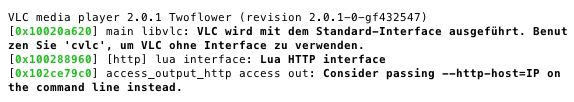
\includegraphics[width=\textwidth]{res/cli-output.jpg}
\caption{VLC Start mit HTTP-Interface}
\label{fig:vlc-start-with-param}
\end{figure}
Hier ist gut sichtbar, dass die HTTP-Requests über das LUA-Interface geleitet werden. Die Aktivierung in den Einstellungen, wie es vor Version 2.x möglich war, existiert nicht mehr. Weiterhin können mit den Parametern  \textit{--http-host \textbf{host}} und \textit{--http-port \textbf{port}} die IP, sowie der Port angegeben werden, unter dem das Interface zu erreichen ist. Um dies zu testen kann man jetzt die Adresse \textit{http://host:port} (Standard: \textit{http:127.0.0.1:8080}) in einem Webbrowser aufrufen und erhält bei Erfolg ein HTML-Interface zur Steuerung. \\
Die einzelnen Bedienelemente senden bei Benutzung eine jQuery-Request an den VLC-Player und benutzt dabei die \textit{command:value} Syntax.
\begin{lstlisting}[caption=Play Button Command][label=code:command_button_query]
$('#buttonPlPlay').click(function(){
					sendCommand({
						'command': 'pl_play',
						'id':$('.jstree-clicked','#libraryTree').first().parents().first().attr('id').substr(5)
					})
					return false;
				});
\end{lstlisting}

\section*{Verfügbare Kommandos}
Da die Dokumentation für die Version ab 2.x sich mit den Commands im Quelltext unterscheidet, werden die aus der Beispielanwendung extrahiert und getestet.
Die folgenden Befehle konnten gefunden werden:\\
\begin{table}
\caption{VLC Command Beschreibung}

\begin{center}
\begin{tabular}{|>{\bfseries}l|c|}
  \hline
  Command & Funktion\\
  \hline\hline
  pl\_play & Playlisteintrag abspielen \\
  pl\_stop & Wiedergabe stoppen \\
  pl\_previous & Einen Titel zurückspringen \\
  pl\_next & Zum nächsten Titel springen \\
  pl\_empty & Playlist leeren \\
  pl\_loop & Loop einschalten \\
  pl\_repeat & Plalisteintrag wiederholen \\
  pl\_random & Zufallsmodus ein/aus \\
  \hline
\end{tabular}
\label{tab:vlc_commands}
\end{center}
\end{table}

Diese Commands sind für den Betrieb des VLC essentiell und werden für die Anfangsphase der Applikationserstellung von größter Wichtigkeit sein. \\
Für die Einstellungen wie Lautstärke oder Seek kann aus dem Quelltext wenig erschlossen werden. Allein die Methoden, um die Werte zu bekommen ist zu finden, sie zu setzen nicht.



\newpage
\nocite{*}
\printbibliography

\listoffigures
\lstlistoflistings
\listoftables

\end{document}

